%%%%%%%%%%%%%%%%%%%%%%%%%%%%%%%%%%%%%%%%%%%%%%%%%%%%%%%%%%%%%%%%%%%%%%%%%%%%%%%%
%
% Template license:
% CC BY-NC-SA 3.0 (http://creativecommons.org/licenses/by-nc-sa/3.0/)
%
%%%%%%%%%%%%%%%%%%%%%%%%%%%%%%%%%%%%%%%%%%%%%%%%%%%%%%%%%%%%%%%%%%%%%%%%%%%%%%%%

%----------------------------------------------------------------------------------------
%	PACKAGES AND OTHER DOCUMENT CONFIGURATIONS
%----------------------------------------------------------------------------------------

\documentclass[
11pt, % The default document font size, options: 10pt, 11pt, 12pt
%oneside, % Two side (alternating margins) for binding by default, uncomment to switch to one side
%chapterinoneline,% Have the chapter title next to the number in one single line
spanish,
singlespacing, % Single line spacing, alternatives: onehalfspacing or doublespacing
%draft, % Uncomment to enable draft mode (no pictures, no links, overfull hboxes indicated)
%nolistspacing, % If the document is onehalfspacing or doublespacing, uncomment this to set spacing in lists to single
%liststotoc, % Uncomment to add the list of figures/tables/etc to the table of contents
%toctotoc, % Uncomment to add the main table of contents to the table of contents
parskip, % Uncomment to add space between paragraphs
%codirector, % Uncomment to add a codirector to the title page
headsepline, % Uncomment to get a line under the header
]{MastersDoctoralThesis} % The class file specifying the document structure



%----------------------------------------------------------------------------------------
%	INFORMACIÓN DE LA MEMORIA
%----------------------------------------------------------------------------------------

\thesistitle{Realidad aumentada para la optimización de procesos industriales} % El títulos de la memoria, se usa en la carátula y se puede usar el cualquier lugar del documento con el comando \ttitle

% Nombre del posgrado, se usa en la carátula y se puede usar el cualquier lugar del documento con el comando \degreename
\posgrado{Carrera de Especialización en Sistemas Embebidos} 
%\posgrado{Carrera de Especialización en Internet de las Cosas} 
%\posgrado{Carrera de Especialización en Intelegencia Artificial}
%\posgrado{Maestría en Sistemas Embebidos} 
%\posgrado{Maestría en Internet de las cosas}

\author{Iván Szkrabko} % Tu nombre, se usa en la carátula y se puede usar el cualquier lugar del documento con el comando \authorname

\director{Mg. Ing. Leandro Lanzieri (FIUBA)} % El nombre del director, se usa en la carátula y se puede usar el cualquier lugar del documento con el comando \dirname
%\codirector{Nombre del codirector (pertenencia)} % El nombre del codirector si lo hubiera, se usa en la carátula y se puede usar el cualquier lugar del documento con el comando \codirname.  Para activar este campo se debe descomentar la opción "codirector" en el comando \documentclass, línea 23.

\juradoUNO{Esp. Ing. Daniel Marquez (FIUBA)} % Nombre y pertenencia del un jurado se usa en la carátula y se puede usar el cualquier lugar del documento con el comando \jur1name
\juradoDOS{Mg. Ing. Roberto Compañy (FIUBA)} % Nombre y pertenencia del un jurado se usa en la carátula y se puede usar el cualquier lugar del documento con el comando \jur2name
\juradoTRES{Mg. Ing. Matías Álvarez (FIUBA)} % Nombre y pertenencia del un jurado se usa en la carátula y se puede usar el cualquier lugar del documento con el comando \jur3name

\ciudad{Ciudad Autónoma de Buenos Aires}
%\ciudad{ciudad de Mendoza}

\fechaINICIO{Junio de 2020}
\fechaFINAL{Junio de 2021}


\keywords{Sistemas embebidos, FIUBA} % Keywords for your thesis, print it elsewhere with \keywordnames


\begin{document}


\frontmatter % Use roman page numbering style (i, ii, iii, iv...) for the pre-content pages

\pagestyle{plain} % Default to the plain heading style until the thesis style is called for the body content


%----------------------------------------------------------------------------------------
%	RESUMEN - ABSTRACT 
%----------------------------------------------------------------------------------------

\begin{abstract}
\addchaptertocentry{\abstractname} % Add the abstract to the table of contents
%
%The Thesis Abstract is written here (and usually kept to just this page). The page is kept centered vertically so can expand into the blank space above the title too\ldots
\centering

En este trabajo se presenta el desarrollo de una aplicación de realidad aumentada para uso industrial. El trabajo surge como una prueba de concepto para la empresa ABB. La aplicación se desarrolló con el fin de mejorar el desempeño de los operadores en la ejecución de procedimientos industriales, típicos en plantas de lubricantes o farmacéuticas, donde la producción tiene que cumplir con un estricto control de calidad.\newline

Para la ejecución del trabajo se utilizaron conceptos de programación orientada a objetos, testing y programación multihilos. También se aplicaron conocimientos referentes al desarrollo de endpoints para la API y gestión de bases de datos. Por otro lado, gracias a la gestión de proyectos, se logró una buena comunicación con los interesados y llevar el control a lo largo de todo el desarrollo. 

\end{abstract}

%----------------------------------------------------------------------------------------
%	CONTENIDO DE LA MEMORIA  - AGRADECIMIENTOS
%----------------------------------------------------------------------------------------

\begin{acknowledgements}
%\addchaptertocentry{\acknowledgementname} % Descomentando esta línea se puede agregar los agradecimientos al índice
\vspace{1.5cm}

Agradezco a mi Director por su apoyo a la investigación y el desarrollo, y a mis Jurados por la evaluación de la presente memoria. 

\end{acknowledgements}

%----------------------------------------------------------------------------------------
%	LISTA DE CONTENIDOS/FIGURAS/TABLAS
%----------------------------------------------------------------------------------------

\tableofcontents % Prints the main table of contents

\listoffigures % Prints the list of figures

\listoftables % Prints the list of tables


%----------------------------------------------------------------------------------------
%	CONTENIDO DE LA MEMORIA  - DEDICATORIA
%----------------------------------------------------------------------------------------

\dedicatory{\textbf{Dedicado a mi familia}}  % escribir acá si se desea una dedicatoria

%----------------------------------------------------------------------------------------
%	CONTENIDO DE LA MEMORIA  - CAPÍTULOS
%----------------------------------------------------------------------------------------

\mainmatter % Begin numeric (1,2,3...) page numbering

\pagestyle{thesis} % Return the page headers back to the "thesis" style

% Incluir los capítulos como archivos separados desde la carpeta Chapters

% Chapter 1

\chapter{Introducción general} % Main chapter title

\label{Chapter1} % For referencing the chapter elsewhere, use \ref{Chapter1} 
\label{IntroGeneral}

%----------------------------------------------------------------------------------------

% Define some commands to keep the formatting separated from the content 
\newcommand{\keyword}[1]{\textbf{#1}}
\newcommand{\tabhead}[1]{\textbf{#1}}
\newcommand{\code}[1]{\texttt{#1}}
\newcommand{\file}[1]{\texttt{\bfseries#1}}
\newcommand{\option}[1]{\texttt{\itshape#1}}
\newcommand{\grados}{$^{\circ}$}

%----------------------------------------------------------------------------------------

%\section{Introducción}

%----------------------------------------------------------------------------------------
En este capítulo se realiza una introducción a la realidad aumentada y los sistemas de control distribuidos. Hacia el final, se explica la motivación, alcance y objetivos del presente trabajo.

\section{Realidad Aumentada}
\subsection{Tecnología}

La digitalización del mundo real tiene distintos niveles. Podemos clasificarla en realidad virtual, realidad aumentada y realidad mixta, como puede verse en la figura \ref{fig:realidades}:

\begin{figure}[htpb]
	\centering
	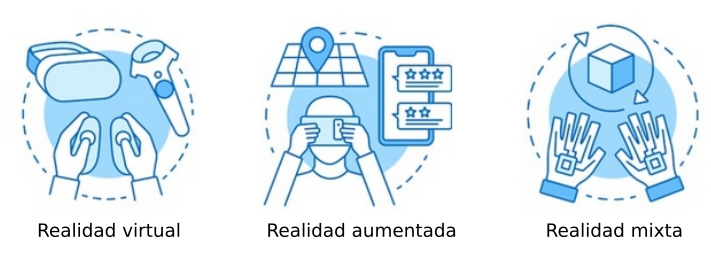
\includegraphics[width=\textwidth]{./Figures/realidades.png}
	\caption{Clasificación de tecnologías\protect\footnotemark.}
	\label{fig:realidades}
\end{figure}

\footnotetext{Imagen tomada de \url{https://scand.com/company/blog/augmented-mixed-and-virtual-reality-for-business/}}

La realidad virtual, consiste en un ambiente completamente digital. Se buscan aislar los sentidos del usuario del mundo real. De esta manera el usuario queda inmerso en otra realidad con la cual puede interactuar. Los dispositivos que permiten esta interacción son los cascos de realidad virtual y sus joysticks.

La realidad aumentada es una tecnología que permite conectar los dos mundos, el mundo físico y el mundo digital. Esto se logra superponiendo imágenes sobre la percepción que tenemos del mundo real, mediante el uso de hologramas o incluso con teléfonos celulares. Donde al activar la cámara, nos muestra en la pantalla no solo el ambiente en el que estamos, sino que vemos proyectada información adicional. Ejemplos de esta tecnología, son los populares filtros de Instagram o el juego PokemonGo.

Por ultimo, la realidad mixta. Esta tecnología es una mejora de la realidad aumentada. Los elementos no solo son adicionados sobre la percepción visual, sino que interactúan ademas con el espacio físico. Por ejemplo, si tuviéramos una pelota en una aplicación de realidad mixta, la misma podría rodar cuesta abajo de una escalera.


\subsection{Procedimientos batch}

Una operación batch o por lotes es aquella en la cual las condiciones de operación cambian con el tiempo. Por lo general, se siguen una serie de pasos, el producto se transfiere a la siguiente fase de la operación, y el proceso comienza de nuevo. En la figura \ref{fig:tanks} podemos ver que en un proceso por lotes, solo cuando llegamos a t=4, obtenemos el producto final deseado:\\

\begin{figure}[htpb]
	\centering
	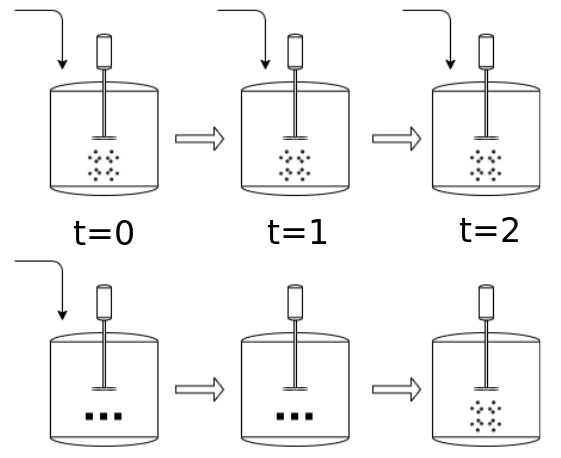
\includegraphics[scale=.45]{./Figures/tanks.png}
	\caption{Proceso continuo (superior) vs. proceso por lotes (inferior)\protect\footnotemark.}
	\label{fig:tanks}
\end{figure}

Los procedimientos operativos para los procesos por lotes son generalmente más complicados y difíciles de escribir que para las instalaciones de estado estacionario porque el tiempo es un factor. Además, muchas instalaciones están diseñadas para fabricar varios productos a partir de los mismos equipamientos en diferentes momentos. Por lo tanto, se necesitan dos o más procedimientos para los mismos equipos de la planta, creando la posibilidad de confusiones y malentendidos.\\

Algunas operaciones por lotes implican el uso de hojas de cálculo. Por ejemplo, un operador puede agregar una bolsa de químicos a un reactor y luego agregar un segundo químico. La razón del segundo al primero debe ser exacta. El operador pesará la primera bolsa, calculará el peso del segundo químico necesario y procederá a pesar ese químico. Se necesita entonces una hoja de cálculo para determinar los requisitos para el peso del segundo producto.

\subsection{Sistemas de control distribuidos}

Los sistema de control distribuidos, también conocidos por sus siglas en ingles DCS. Son sistemas compuestos por sensores, controladores y computadoras que se distribuyen por toda la planta. Cada uno de estos elementos tiene un propósito único, como la adquisición de datos, el control de procesos, el almacenamiento de datos o la visualización gráfica. Estos elementos individuales se comunican con una sistema centralizado a través de la red de área local de la planta, denominada red de control. A continuación se muestra en la figura \ref{fig:800xA}, la arquitectura de red del sistema DCS de ABB, usado en este trabajo:

\begin{figure}[htpb]
	\centering
	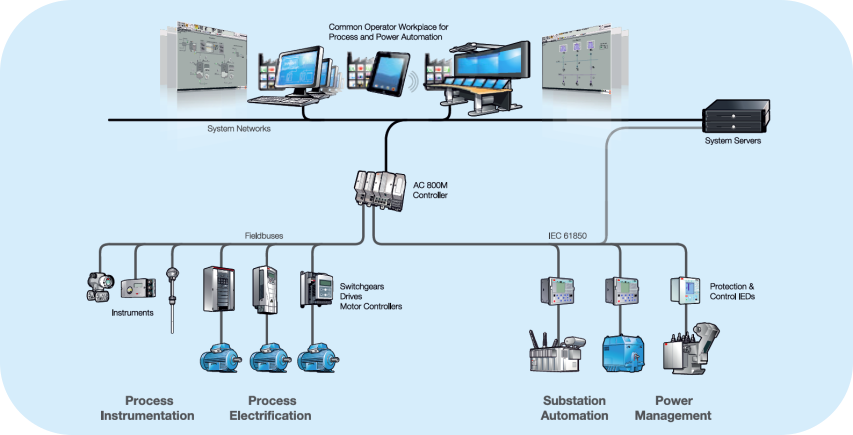
\includegraphics[width=\textwidth]{./Figures/800xA.png}
	\caption{Sistema de control distribuido 800xA\protect\footnotemark.}
	\label{fig:800xA}
\end{figure}

\footnotetext{Imagen tomada de \url{https://new.abb.com/control-systems/system-800xa/800xa-dcs/system/architecture}}

El DCS toma decisiones automatizadas basadas en las tendencias de producción de toda la planta. Como ejemplo, el DCS de una planta de energía, podría aumentar automáticamente la capacidad de generación de vapor de múltiples turbinas, para adecuarse a la demanda cambiante de electricidad. Mientras que un PLC puede ajustar la operación de una sola unidad, el DCS puede realizar ajustes en cada una de las unidades de control que interactúan en una planta.

\subsection{Protocolo OPC}

OPC (Open Platform Communications) es el estándar de interoperatividad para el intercambio seguro y confiable de datos en la industria. Tiene especial uso en los DCS, dado que son sistemas compuestos por productos de distintos rubros y fabricantes. El protocolo es independiente de la plataforma y garantiza el flujo continuo de información entre dispositivos de múltiples proveedores. La Fundación OPC es responsable del desarrollo y mantenimiento de este estándar. Estas especificaciones definen el acceso a datos en tiempo real, monitoreo de alarmas y eventos, acceso a datos históricos y otras aplicaciones. 

%----------------------------------------------------------------------------------------
\subsection{Otros trabajos}

\subsubsection{Smart retrofitting in the context of industry 4.0}
En este trabajo publicado en Elsevier (CIRP 88 369–374), se utiliza el Hololens para capacitar a los operadores luego de una mejora en una maquina dobladora de caños. El trabajo destaca que la herramienta permite a los operadores adaptarse rápidamente a la maquina, permitiéndoles trabajar de manera segura y guiada.

\subsubsection{Production workplace enhanced by mixed reality}
En este paper presentado en la conferencia Mensch und Computer 2020 en Alemania (muc2020-ws116-005), se muestra una aplicación de realidad aumentada para guiar al operador en el ensamblado de un scooter. El trabajo destaca el análisis de la relación costo-beneficio a la hora de armar procedimientos para los operadores. Plantea que deben evaluarse, el tiempo y presupuesto para el desarrollo del procedimiento, en comparación con el costo de una falla de ensamblado.

\subsubsection{Mixed reality technology for onsite construction assembly}
En este paper presentado en la conferencia Materials Science, Engineering and Chemistry 2020 (Matec 312,06001), se presenta una aplicación de realidad aumentada cuyo objetivos es comunicar los detalles de diseño para el montaje y la construcción. El trabajo destaca que el Hololens es capaz de guiar la instalación de componentes eléctricos y de plomería, logrando un 9\% de mejora en la productividad. Menciona ademas, que las imágenes ocluidas en condiciones de luz solar, son el desafió a superar por el HoloLens antes de una adopción generalizada.

\section{Motivación}
El propósito de este proyecto es innovar en la interacción entre los operadores y los sistema de control distribuidos, para impulsar nuevas soluciones en el área de la automatización industrial. Se busca explorar las oportunidades que ofrece la realidad aumentada para mejorar y optimizar las tareas de los operadores, además de agilizar el entrenamiento de nuevos operarios y mejorar la seguridad para procedimientos bajo situaciones de emergencia.

%----------------------------------------------------------------------------------------

\section{Alcance}

En la presente memoria, se documenta el trabajo realizado donde se incluyen los siguientes aspectos:

\begin{itemize}	
\item Desarrollo de la aplicación de realidad aumentada.
\item Desarrollo del conector OPC.
\item Desarrollo de API REST.
\item Comunicación entre el DCS y la interfaz holográfica.
\item Implementación de base de datos cloud.
\end{itemize}
\chapter{Introducción específica} % Main chapter title

\label{Chapter2}

%----------------------------------------------------------------------------------------
%	SECTION 1
%----------------------------------------------------------------------------------------
En este capítulo se presentan las herramientas usadas para desarrollar el trabajo y un breve compendio de otros trabajos similares en la temática. Hacia el final, se encuentran los requerimientos y la planificación utilizada.

\section{Entorno de desarrollo}
\subsection{Hololens2}

El equipo que se utilizó para la interfaz de realidad aumentada es el Microsoft Hololens 2. Podemos ver una foto del equipo en la figura \ref{fig:hololens2}:

\begin{figure}[htpb]
	\centering
	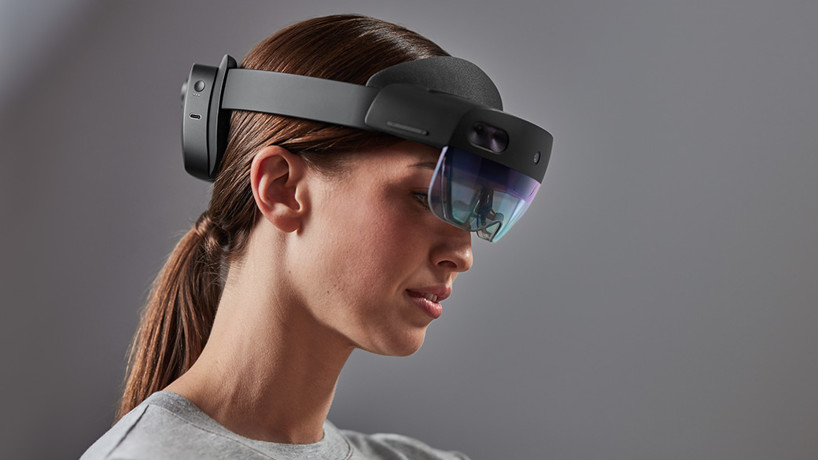
\includegraphics[scale=.5]{./Figures/hololens2.jpeg}
	\caption{Hololens 2\protect\footnotemark.}
	\label{fig:hololens2}
\end{figure}

\footnotetext{Imagen tomada de \url{https://img-prod-cms-rt-microsoft-com.akamaized.net/cms/api/am/imageFileData/}}


Fue lanzado al mercado para uso corporativo, Microsoft apuesta a que la tecnología sea usada con fines productivos en distintas industrias. Es un equipo de última generación que funciona con un sistema operativo Windows 10 core.  La tabla \ref{tab:holotab}, muestra sus especificaciones técnicas.

\begin{table}[htpb]
	\centering
	\caption[Hardware Hololens 2]{Especificaciones técnicas Hololens 2}
	\scalebox{0.9}{
	\begin{tabular}{l c c}    
		\toprule
		\textbf{Hardware} 	 & \textbf{Descripción}  \\
		\midrule
		Procesador				&  Qualcomm Snapdragon 850 \\		
		Memoria	 				&  4 GB DRAM \\
		Almacenamiento	 		&   64 GB \\
		Cámara	 				&   1080p \\
		Peso 	 				&   566 gr \\
		CPU holográfica			&   Segunda generación\\
		Resolución				&   2k 3:2\\
		Unidad de medida inercial			&   Acelerómetro, giroscopio y magnetómetro\\
		Seguimiento de cabeza	&   4 cámaras de luz visible\\
		Seguimiento de ojos	&   2 cámaras de infrarrojas\\
		\bottomrule
		\hline
	\end{tabular}}
	\label{tab:holotab}
\end{table}

Lo innovador de su diseño es que utiliza micro espejos para proyectar tres haces de luz láser de color rojo, verde y azul. Con un micro espejo por cada ojo oscilando a 12.000 veces por segundo, compone la imagen horizontal. Con un segundo micro espejo, oscilando a 120 veces por segundo forma la componente vertical. Luego,este haz de luz es proyectado hacia nuestra retina, utilizando el visor del Hololens 2 que actúa como una guía de onda. En la figura \ref{fig:Lasers} podemos ver una ejemplificación del funcionamiento interno:

\begin{figure}[htpb]
	\centering
	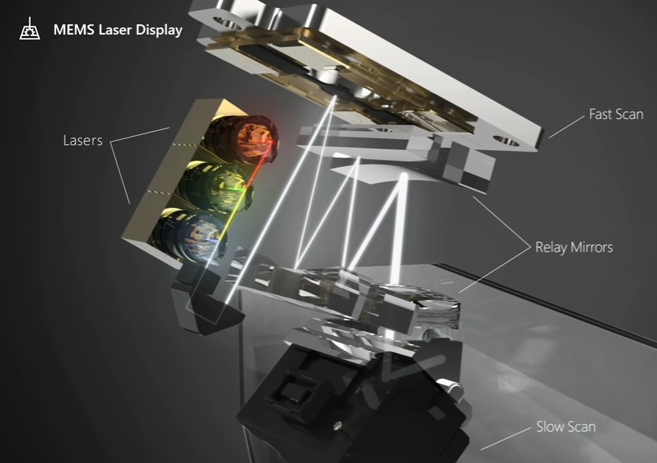
\includegraphics[width=\textwidth]{./Figures/Lasers.png}
	\caption{Micro espejos\protect\footnotemark.}
	\label{fig:Lasers}
\end{figure}

\footnotetext{Imagen tomada de \url{https://img-prod-cms-rt-microsoft-com.akamaized.net/cms/api/am/imageFileData/}}


\subsection{MRTK}

MRTK (\textit{Mixed Reality Toolkit}) para Unity es un kit de desarrollo multiplataforma de código abierto para aplicaciones de realidad mixta. Proporciona un sistema de entrada, componentes fundamentales y bloques de construcción comunes para interacciones espaciales. Tiene como objetivo acelerar el desarrollo de aplicaciones para Microsoft HoloLens 2, los visores inmersivos de Windows Mixed Reality y la plataforma OpenVR. El proyecto busca reducir las barreras de entrada, crear aplicaciones de realidad mixta y contribuir a la comunidad. El \textit{framework} puede desglosarse conceptualmente como se muestra en la \ref{fig:mrtk}:

\begin{figure}[htpb]
	\centering
	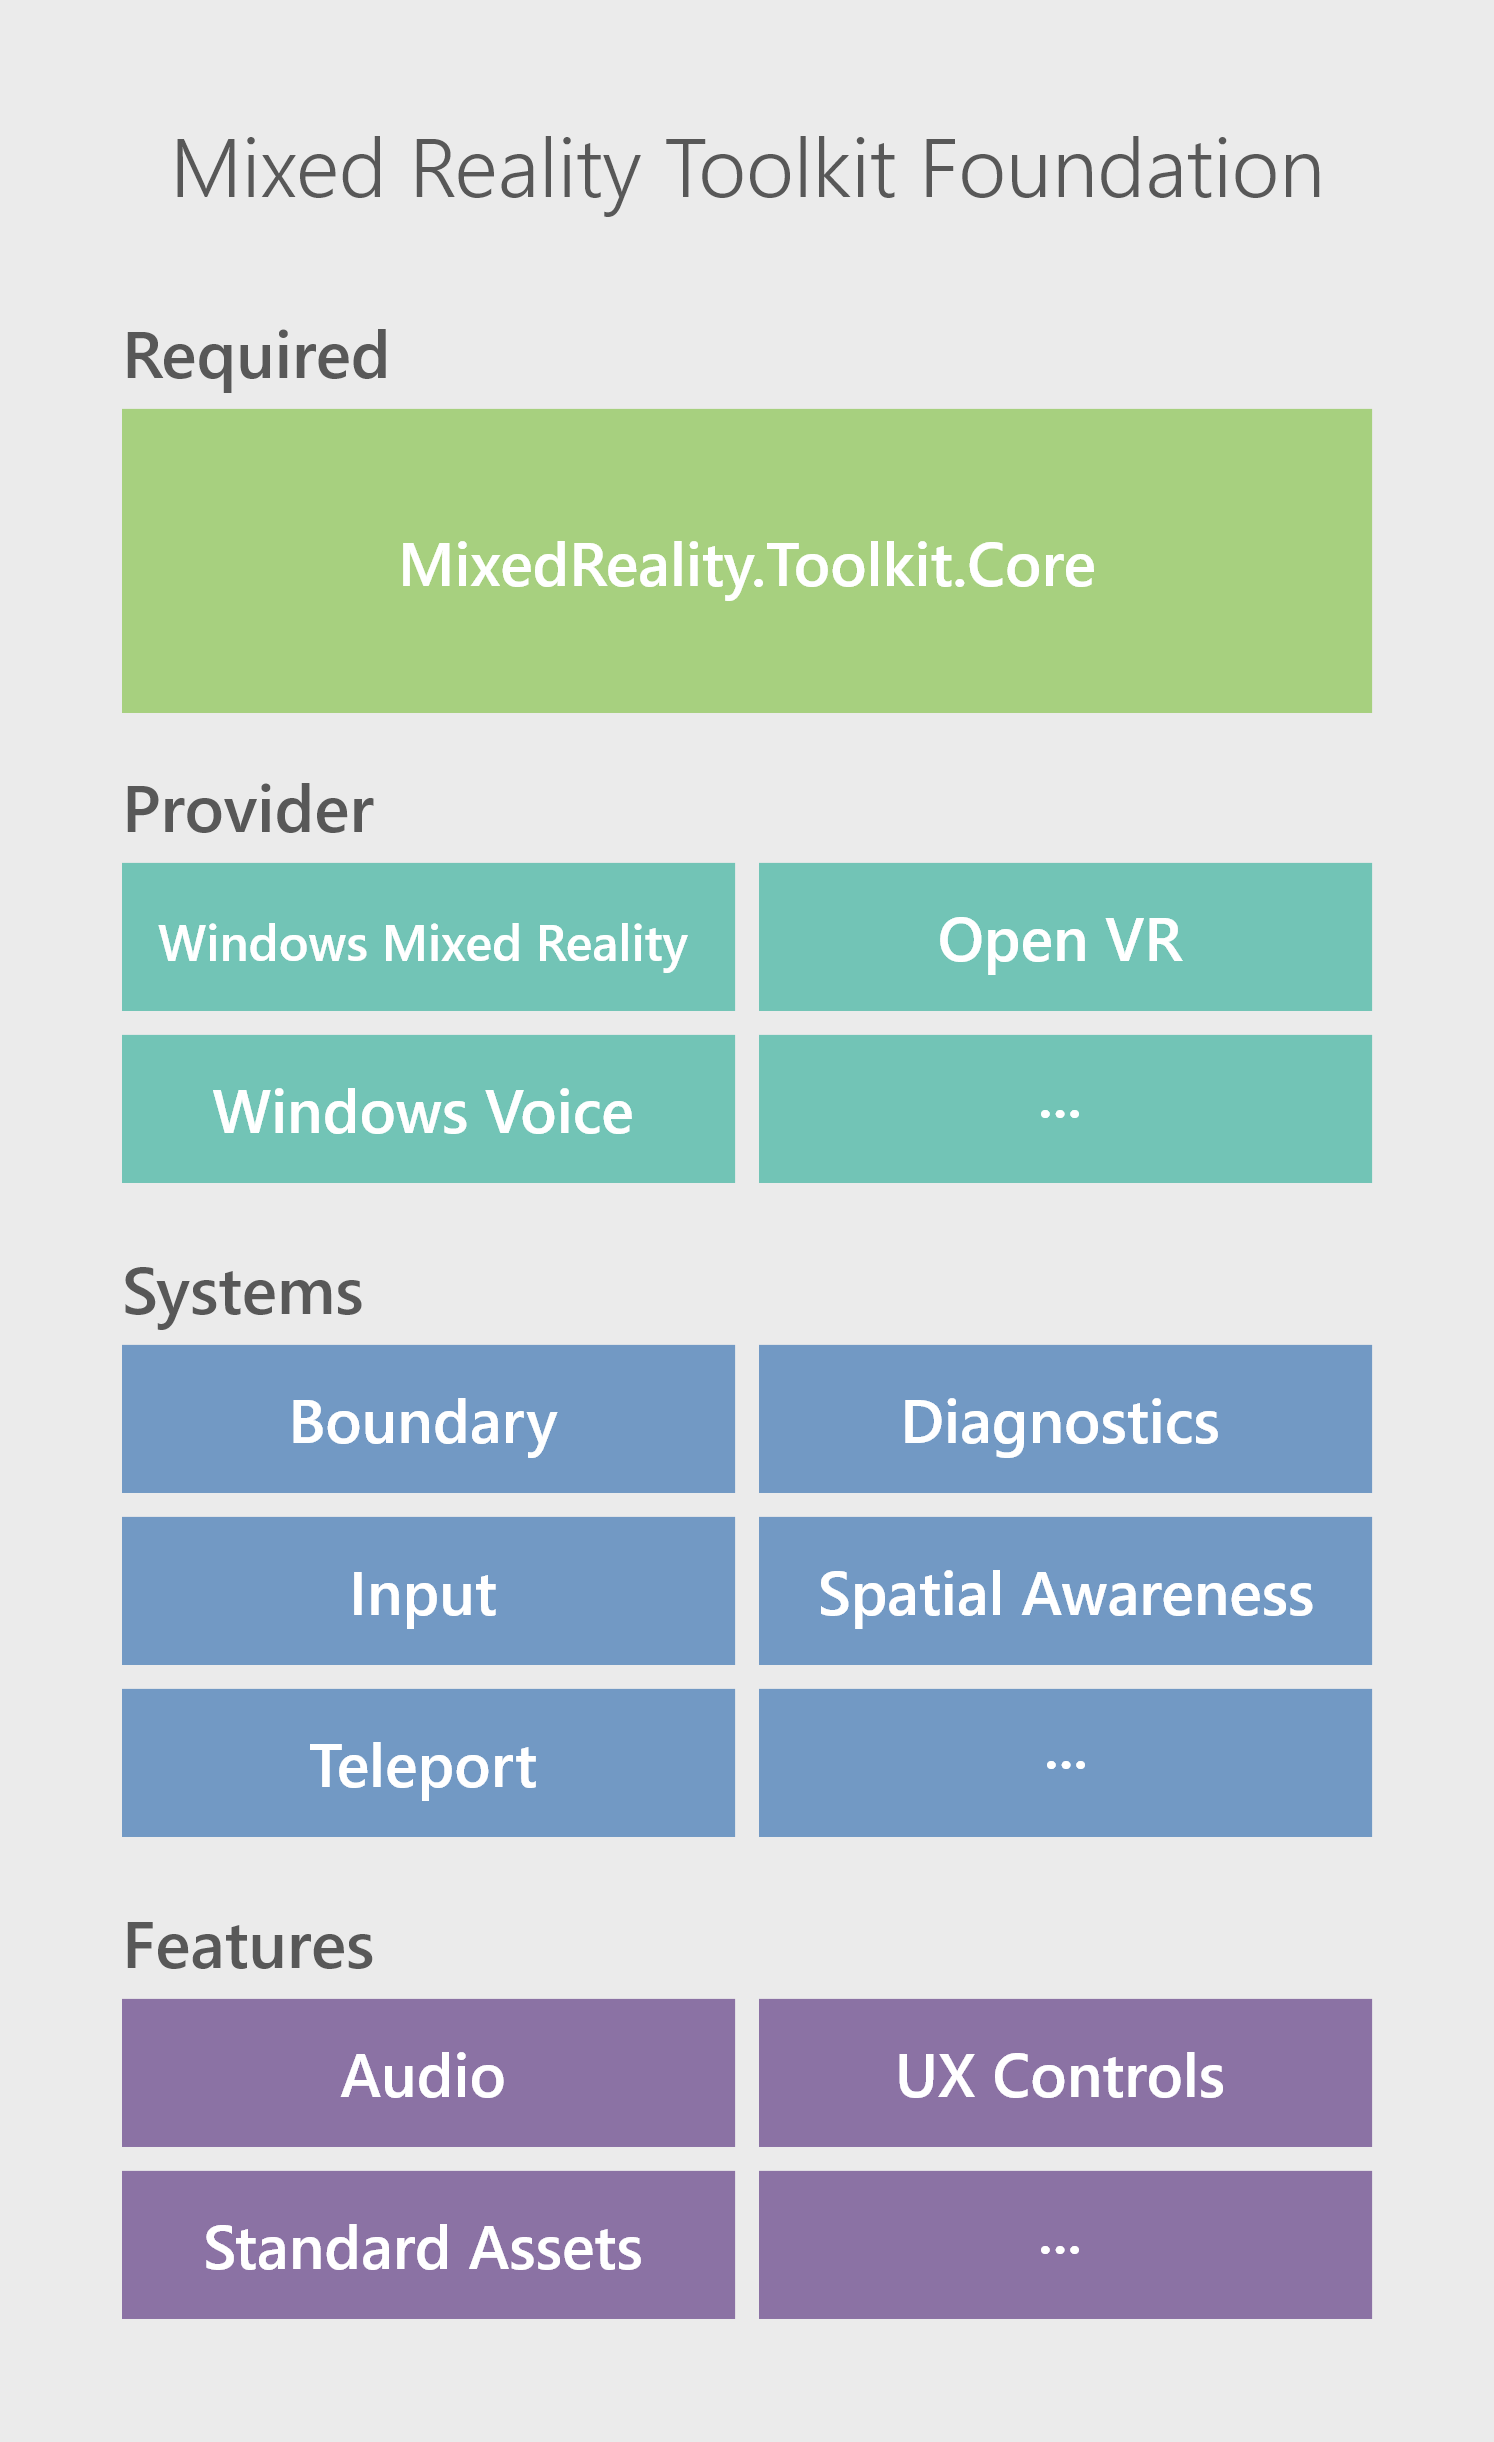
\includegraphics[scale=0.14]{./Figures/mrtk.png}
	\caption{Componentes del MRTK \textit{framework}\protect\footnotemark.}
	\label{fig:mrtk}
\end{figure}

\footnotetext{Imagen tomada de \url{https://docs.microsoft.com/en-us/windows/mixed-reality/}}

Sus componentes principales son:
\begin{itemize}
\item \textit{Hands}: clase básica de soporte con servicios para seguimiento de las manos.
\item \textit{ObjectMeshObserver}: procesamiento del ambiente usando el modelado 3D.
\item \textit{WindowsMixedReality}: compatibilidad con dispositivos \textit{Windows Mixed Reality}, incluidos Microsoft HoloLens y auriculares inmersivos.
\item \textit{Profiles}: perfiles predeterminados para los sistemas y servicios de \textit{Microsoft Mixed Reality Toolkit}.
\item \textit{SceneSystem}: sistema que proporciona compatibilidad con aplicaciones de múltiples escenas.
\item \textit{StandardAssets}: renderizado estándar, materiales básicos y otros activos para experiencias de realidad mixta.
\end{itemize}

Además del MRTK, se utilizan programas de diseño como el Fusion360 para crear objetos 3D. Se utiliza el Visual Studio como IDE de desarrollo y como herramienta de compilación. Y finalmente Unity, como herramienta de diseño visual de la aplicación. En la figura \ref{fig:workflow}, podemos ver un diagrama del entorno completo:

\begin{figure}[htpb]
	\centering
	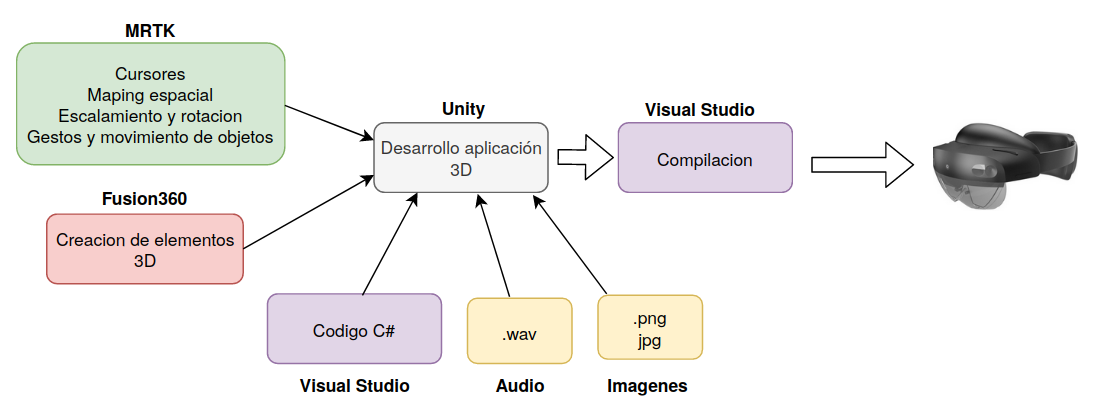
\includegraphics[scale=0.44]{./Figures/workflow.png}
	\caption{Entorno de desarrollo\protect\footnotemark.}
	\label{fig:workflow}
\end{figure}

\vspace{10px}

\footnotetext{Imagen tomada de \url{https://img-prod-cms-rt-microsoft-com.akamaized.net/cms/api/am/imageFileData/}}

\subsection{OPC \textit{framework}}

Las especificaciones de OPC \textit{Classic} se basan en la tecnología de Microsoft Windows, utilizando COM / DCOM (\textit{Distributed Component Object Model}) para la comunicación entre componentes de software en una red distribuida cliente-servidor. La especificación original es OPC-DA (\textit{Data Access}), que define una interfaz entre las aplicaciones cliente y servidor para intercambiar datos de proceso y fabricación. Antes de OPC-DA, los productos de distintos proveedores (PLC, HMI) requerían que cualquier dispositivo o aplicación que se conectara a ellos, tuviera un ``controlador personalizado'' que comunicara el dispositivo con equipos de terceros. En la figura \ref{fig:OPCAQ} se muestra una arquitectura típica de control previa a la existencia del \textit{standard} OPC.

\begin{figure}[htpb]
	\centering
	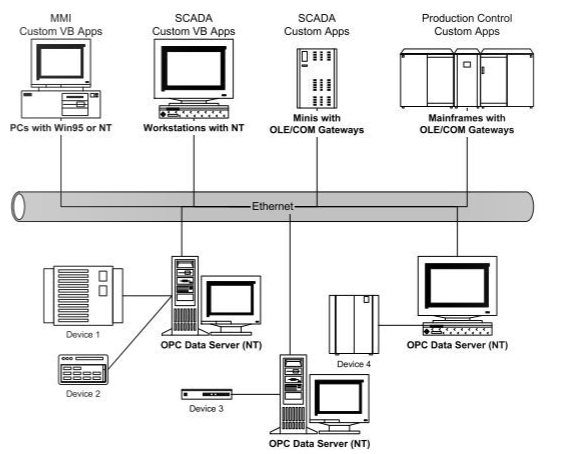
\includegraphics[scale=0.7]{./Figures/opc_1.png}
	\caption{Arquitectura OPC\protect\footnotemark.}
	\label{fig:OPCAQ}
\end{figure}

\footnotetext{Imagen tomada de \url{https://technosoftware.com/opc-daaehda-client-net}}

Hubo muchos problemas asociados con las comunicaciones basadas en controladores personalizados. La tecnología patentada de alto costo que forzaba a los usuarios a mantener un proveedor en particular. Dificultades para configurar y  mantener actualizado los \textit{drivers} debido al lanzamiento de nuevos dispositivos y aplicaciones. OPC-DA hizo posible la conexión a cualquier fuente de datos en tiempo real sin un driver escrito específicamente para el par fuente de datos / receptor de datos. Por lo tanto, las lecturas y escrituras se pueden realizar sin que el receptor de datos tenga que conocer el protocolo nativo de la fuente de datos o la estructura de datos interna.\\ 

La especificación describe los objetos y sus interfaces, las cuales son implementadas por los servidores OPC. Aunque OPC está diseñado principalmente para acceder a datos desde un servidor en red, las interfaces se pueden utilizar en muchos lugares dentro de una aplicación. En el nivel más bajo, pueden obtener datos sin procesar de los dispositivos físicos y enviarlos a un SCADA o DCS, o desde el sistema SCADA o DCS a la aplicación. La arquitectura y el diseño permiten que una aplicación cliente acceda a datos de muchos servidores OPC proporcionados por distintos proveedores. En la figura \ref{fig:OPCbloques} se muestra un diagrama en bloques para ejemplificar lo explicado:

\begin{figure}[htpb]
	\centering
	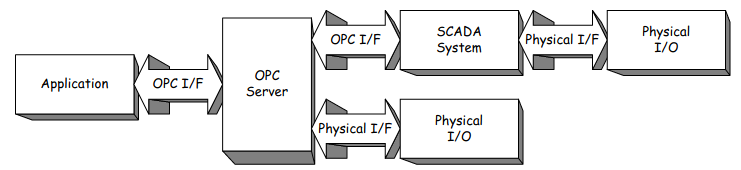
\includegraphics[scale=0.5]{./Figures/opc_2.png}
	\caption{Diagrama en bloques\protect\footnotemark.}
	\label{fig:OPCbloques}
\end{figure}

\footnotetext{Imagen tomada de \url{https://opcfoundation.org}}

A alto nivel, un servidor OPC se compone de varios objetos: el servidor, el grupo y el elemento. El objeto del servidor OPC mantiene información sobre el servidor y sirve como contenedor para los objetos del grupo. El objeto del grupo mantiene información sobre sí mismo y proporciona el mecanismo para contener y organizar lógicamente los elementos OPC. Un cliente se comunica con el servidor a través de las interfaces para cada objeto OPC, como se ve en la figura \ref{fig:OPCapi}.

\begin{figure}[htpb]
	\centering
	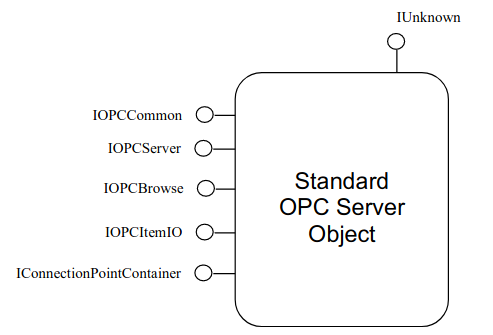
\includegraphics[scale=0.4]{./Figures/opc_3.png}
	\caption{Objeto OPC\protect\footnotemark.}
	\label{fig:OPCapi}
\end{figure}

\footnotetext{Imagen tomada de \url{https://opcfoundation.org}}

\begin{itemize}
\item IOPC Server: ésta es la interfaz principal de un servidor OPC, permite realizar las consultas a los grupos de elementos OPC.
\item IUnknown: consiste en un puntero a una tabla que permite descubrir dinámicamente si un objeto admite una interfaz en particular.
\item IOPC Common:Proporciona la capacidad de configurar y consultar el LocaleID para la sesión cliente/servidor en particular. El LocaleID contempla el formato de números, fechas, moneda, etc. Puede depender de la configuración regional.
\item IOPC Browse: proporciona métodos mejorados para navegar por el espacio de direcciones del servidor y para
obtener propiedades de los elementos OPC.
\item IConnectionPointContainer: permite disparar eventos llamando a un método de la interfaz de un objeto COM del lado del cliente implementado por el mismo cliente.
\item IOPC ItemIO: en términos de rendimiento esta interfaz se comportará como si se creara un grupo, se agregaran los elementos OPC, se realizará una sola lectura o escritura y luego se eliminará el grupo. Por lo tanto no es la interfaz recomendada para la mayoría de las aplicaciones.
\end{itemize}

Los grupos OPC proporcionan una forma para que los clientes organicen los datos. Por ejemplo, el grupo puede representar elementos en una pantalla de operación o variables de un lazo PID. Los datos se pueden leer y escribir. Los elementos OPC representan conexiones a fuentes de datos dentro del servidor. Un elemento OPC, desde la perspectiva de la interfaz, no es accesible como objeto por un cliente OPC. Por lo tanto, no hay una interfaz externa definida para un elemento OPC. Todo el acceso a los elementos OPC se realiza a través de un objeto de grupo que contiene los elementos. Un grupo también proporciona una forma para que el cliente se ``suscriba'' a la lista de elementos para que pueda ser notificado cuando cambien. Este ratio de actualización es un parámetro configurable del servidor.


\section{Requerimientos}

A continuación se listan los requerimientos en base a las distintas etapas del trabajo:

\begin{enumerate}
\item Requerimientos asociados al desarrollo de la interfaz visual:
	\begin{enumerate}
	\item La interfaz debe ser intuitiva y simple.
	\item El idioma definido es Español.
	\end{enumerate}
\item Requerimientos asociados al desarrollo de lógica en .NET:
	\begin{enumerate}
	\item La aplicación debe ser fluida y responder sin demoras apreciables por el operador, estableciéndose así el límite máximo de espera en 2 segundos.
	\item La aplicación debe poder hacer operaciones GET y POST sobre un servidor web, ya sea local o en la nube.
	\end{enumerate}
\item Requerimientos asociados a la API rest:
	\begin{enumerate}
	\item La API no será de acceso público, solo podrá ser consultada por las aplicaciones que poseen un \textit{token} de seguridad.
	\end{enumerate}
\item Requerimientos asociados a la interfaz de comunicación con el sistema de control:	
	\begin{enumerate}	
	\item La solución debe poder consultar una serie de datos específicos a elección, de los elementos que pertenecen al sistema de control.
	\item La comunicación debe cumplir con el \textit{standard} OPC.
	\end{enumerate}
\end{enumerate}

\section{Planificación}

El trabajo fue dividido en tareas y se estimaron los tiempos que debían emplearse para cada una de ellas. A su vez, se analizaron qué tareas debían realizarse primero y cuáles eran sus dependencias. Al momento de organizar las tareas se consideraron 15 horas semanales efectivas de trabajo, obteniendo como resultado la planificación de la figura \ref{figure:gantt}:

\begin{figure}[htpb]
	\centering
	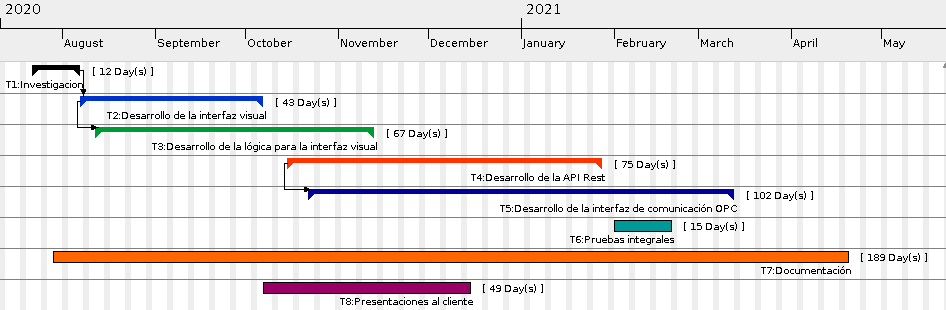
\includegraphics[width=14cm]{./Figures/gantt_1.png}
	\caption{Diagrama de Gantt\protect\footnotemark.}
	\label{figure:gantt}
\end{figure}

Como se estimó al inicio del trabajo, la comunicación OPC fue la que más tiempo empleó, incluso se extendió un mes más de lo planeado.  
\chapter{Diseño e implementación} % Main chapter title

\label{Chapter3} % Change X to a consecutive number; for referencing this chapter elsewhere, use \ref{ChapterX}

\definecolor{mygreen}{rgb}{0,0.6,0}
\definecolor{mygray}{rgb}{0.5,0.5,0.5}
\definecolor{mymauve}{rgb}{0.58,0,0.82}

%%%%%%%%%%%%%%%%%%%%%%%%%%%%%%%%%%%%%%%%%%%%%%%%%%%%%%%%%%%%%%%%%%%%%%%%%%%%%
% parámetros para configurar el formato del código en los entornos lstlisting
%%%%%%%%%%%%%%%%%%%%%%%%%%%%%%%%%%%%%%%%%%%%%%%%%%%%%%%%%%%%%%%%%%%%%%%%%%%%%
\lstset{ %
  backgroundcolor=\color{white},   % choose the background color; you must add \usepackage{color} or \usepackage{xcolor}
  basicstyle=\footnotesize,        % the size of the fonts that are used for the code
  breakatwhitespace=false,         % sets if automatic breaks should only happen at whitespace
  breaklines=true,                 % sets automatic line breaking
  captionpos=b,                    % sets the caption-position to bottom
  commentstyle=\color{mygreen},    % comment style
  deletekeywords={...},            % if you want to delete keywords from the given language
  %escapeinside={\%*}{*)},          % if you want to add LaTeX within your code
  %extendedchars=true,              % lets you use non-ASCII characters; for 8-bits encodings only, does not work with UTF-8
  %frame=single,	                % adds a frame around the code
  keepspaces=true,                 % keeps spaces in text, useful for keeping indentation of code (possibly needs columns=flexible)
  keywordstyle=\color{blue},       % keyword style
  language=[ANSI]C,                % the language of the code
  %otherkeywords={*,...},           % if you want to add more keywords to the set
  numbers=left,                    % where to put the line-numbers; possible values are (none, left, right)
  numbersep=5pt,                   % how far the line-numbers are from the code
  numberstyle=\tiny\color{mygray}, % the style that is used for the line-numbers
  rulecolor=\color{black},         % if not set, the frame-color may be changed on line-breaks within not-black text (e.g. comments (green here))
  showspaces=false,                % show spaces everywhere adding particular underscores; it overrides 'showstringspaces'
  showstringspaces=false,          % underline spaces within strings only
  showtabs=false,                  % show tabs within strings adding particular underscores
  stepnumber=1,                    % the step between two line-numbers. If it's 1, each line will be numbered
  stringstyle=\color{mymauve},     % string literal style
  tabsize=2,	                   % sets default tabsize to 2 spaces
  title=\lstname,                  % show the filename of files included with \lstinputlisting; also try caption instead of title
  morecomment=[s]{/*}{*/}
}


%----------------------------------------------------------------------------------------
%	SECTION 1
%----------------------------------------------------------------------------------------
\section{Análisis del software}

\subsection{Arquitectura del sistema}
La solución está integrada por seis componentes principales:

\begin{itemize}
\item Interfaz visual: diseñada en Unity3D, le permite al usuario interactuar con la aplicación.
\item Lógica .NET: es el backend de la interfaz visual, es la aplicación desarrollada en .NET utilizando CSharp como lenguaje de programación.
\item APIrest: a través de ella la aplicación embebida en el Hololens 2 se comunica con el servidor web.
\item Base de datos: es actualizada a través de la APIrest y almacena los parámetros del proceso \textit{batch}.
\item Comunicación OPC: envía los datos pertinentes al sistema de control a través del \textit{standard} industrial OPC.
\item Sistema de control: es representado por un controlador simulado.
\end{itemize}

En la figura \ref{fig:Diag_bloques} se puede observar el diagrama en bloques y la interacción entre los seis componentes principales.

\begin{figure}[htpb]
	\centering
	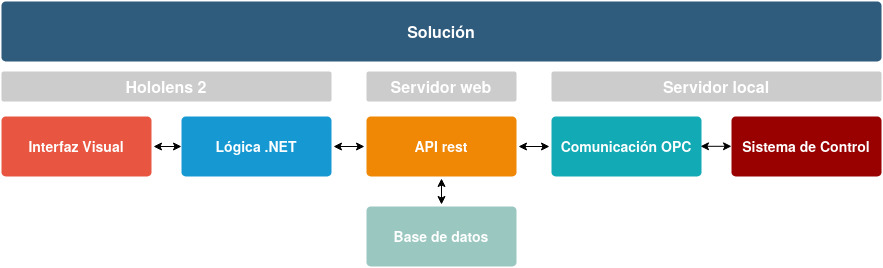
\includegraphics[scale=.5]{./Figures/Diag_bloques.jpg}
	\caption{Diagrama en bloques del sistema\protect\footnotemark.}
	\label{fig:Diag_bloques}
\end{figure}

\subsection{Interfaz visual y lógica .NET}

La aplicación embebida en el Hololens 2 se encarga de guiar al operador a través de todo el procedimiento \textit{batch}. En la figura \ref{fig:Flujo} se puede ver el diagrama de flujo.

\begin{figure}[htpb]
	\centering
	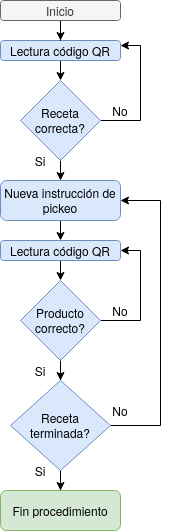
\includegraphics[scale=.7]{./Figures/Flujo.png}
	\caption{Diagrama de flujo\protect\footnotemark.}
	\label{fig:Flujo}
\end{figure}

En términos generales la aplicación se basa en la lectura de códigos QR para poder validar la operatoria del usuario. De esta manera, a lo largo del procedimiento se le solicitaran al operador distintas tareas las cuales tendrán asociadas un código QR especifico. Por ejemplo, para el agregado de un insumo al tanque de producción, se solicitara la lectura del código de la bolsa del insumo correcto para poder continuar. Mientras que en un proceso de transvase entre tanques, se le solicitara la lectura del código de la válvula que debe actuar para poder continuar. Como se muestra en la figura \ref{fig:Flujo}, mientras la lectura no sea correcta el operador no podrá avanzar de etapa.

A mas bajo nivel, cuando la aplicación inicia se instancia el objeto QRwatcher y el objeto Post. QRwatcher se ejecuta en \textit{background} para detectar la presencia de códigos QR en el ambiente, utilizando la cámara frontal del Hololens 2. Ademas crea una interfaz de servicio, para que el objeto Post se registre al mismo y reciba un \textit{handler} cuando ocurre una detección. El objeto Post se encarga de realizar las consultas a la API y crea el objeto Navegacion, este actualiza la información mostrada al operador durante todo el procedimiento. 

Luego de una detección, el \textit{handler} devuelve el dato codificado de la imagen QR y las coordenadas espaciales del código leído. Utilizando estas coordenadas se instancia un elemento holográfico, para indicar al operador si el código leído es correcto o incorrecto. Para esto se utilizo un tilde verde o una cruz roja sobre el código leído. De acuerdo con el tipo de lectura se dinamizan también botones alrededor del código. 

Utilizando los botones holográficos el operador puede cancelar la lectura o aceptarla. Si el código es incorrecto sólo podrá cancelar la lectura. Los botones tienen asociados eventos que disparan \textit{callbacks} al detectarse el pulsado. Si la lectura es correcta, el operador oprimirá aceptar y el \textit{callback} destruirá las instancias holográficas creadas, haciendo desaparecer los botones de la visual del operador. Al mismo tiempo, incrementa la variable de referencia \textit{steps}. Esta variable es publica del objeto Navegacion y se utiliza para determinar en que paso se encuentra la receta. El objeto Navegacion internamente implementa una maquina de estados para indicarle al operador las instrucciones correspondientes en cada etapa. 

En la etapa inicial, el objeto Post se encarga de ejecutar una consulta a la API y traer todos los parámetros de la receta leída. Estos parámetros se guardan en un objeto dataReceta el cual permanece inmutable durante toda la aplicación. Con estos datos, el objeto Navegacion es capaz de solicitar las instrucciones correctas en cada etapa e identificar cual seria el código requerido en cada una para poder avanzar. A continuación se muestra la maquina de estados del objeto Navegacion:

\begin{lstlisting}[label=cod:vControl,caption=Maquina de estados]  % Start your code-block

switch (steps)
{
	case 1:
   	textoinstruccion.GetComponent<TMPro.TextMeshProUGUI>().text = POST.dataReceta.msg1;
    break;
	
	case 2:
    _ = POST.PatchAsync("ValidationS1", "1");
    textoinstruccion.GetComponent<TMPro.TextMeshProUGUI>().text = POST.dataReceta.msg2;
    break;

	case 3:
    _ = POST.PatchAsync("ValidationS2", "1");
    textoinstruccion.GetComponent<TMPro.TextMeshProUGUI>().text = POST.dataReceta.msg3;
    break;

    case 4:
    _ = POST.PatchAsync("ValidationS3", "1");
    textoinstruccion.GetComponent<TMPro.TextMeshProUGUI>().text = POST.dataReceta.msgEnd;
    ButtonDatos.SetActive(false);
    canvas_proc.SetActive(false);
    ButtonMostrar.SetActive(false);
    MsgFin.SetActive(true);
    break;

    default:
    break;
}
\end{lstlisting}

La ventaja de esta solución es que el usuario puede modificar los códigos y las instrucciones requeridas sin interferir en la lógica de la aplicación dado que cada etapa se encuentra parametrizada con la información almacenada en la base de datos.

\subsection{API y base de datos}
La API (\textit{Application Programming Interface}) fue desarrollada en .NET y se implementaron las siguientes operaciones:

\begin{itemize}
\item GET: devuelve los datos de una receta.
\item POST: permite crear nuevas recetas.
\item PATCH: permite actualizar ciertos campos de la receta sin alterar el resto.
\item DELETE: elimina recetas de la colección.
\end{itemize}

Se creó una clase ``Receta'' la cual contiene los siguientes parámetros:

\begin{itemize}
\item id: número de identificación de la receta.
\item Receta: producto a fabricar.
\item Descripción: descripción del producto.
\item Status: running o stop, indica el estado de la receta.
\item Waitinput: sólo si esta en 1 la receta aguarda input del operador.
\item ValidationS1: 1 o 0 dependiendo si se cumplió la etapa del procedimiento.
\item ValidationS2: 1 o 0 dependiendo si se cumplió la etapa del procedimiento.
\item ValidationS3: 1 o 0 dependiendo si se cumplió la etapa del procedimiento.
\item ProductoP1: Nombre del producto de la etapa 1.
\item ProductoP2: Nombre del producto de la etapa 2.
\item ProductoP3: Nombre del producto de la etapa 3.
\item CodigoP1: Código del producto de la etapa 1.
\item CodigoP2: Código del producto de la etapa 2.
\item CodigoP3: Código del producto de la etapa 3.
\item CantidadP1: Cantidad del producto de la etapa 1.
\item CantidadP2: Cantidad del producto de la etapa 2.
\item CantidadP3: Cantidad del producto de la etapa 3.
\item Msg1: Mensaje para la etapa 1.
\item Msg2: Mensaje para la etapa 2.
\item Msg3: Mensaje para la etapa 3.
\item MsgEnd: Mensaje de fin de proceso.
\end{itemize}

Esta clase también se implementó en la lógica del Hololens 2. De esta manera, se utilizan los métodos GET y PATCH durante los pasos de la interfaz para adquirir o enviar datos a la API. Cuando desde la interfaz se lee un código QR internamente se envía una petición GET al servidor web para traer los datos de la receta y almacenarlos en una instancia de la clase Receta. Si la receta es correcta, se utiliza el mismo ID de receta para enviar las actualizaciones de estado cuando el operador avance una etapa. Esta actualización se hace con el método PATCH. Éste se implementó para modificar sólo los parámetros del input de usuario en la receta y no alterar el resto. 

La API se hosteo en Azure, la plataforma \textit{cloud} de Microsoft \citep{Azure}. Se utilizó el servicio Azure Web Apps \citep{WebApps}, que es una plataforma que permite publicar aplicaciones web que se ejecutan en múltiples \textit{frameworks} y escritas en diferentes lenguajes de programación. Esto permitió aumentar la velocidad de desarrollo de la aplicación dado que la sincronización y el \textit{deployment} son prácticamente instantáneos. Además, ofrece múltiples posibilidades de integración con otros servicios a futuro.

El motor de la base de datos utilizado es MongoDB \citep{mongo}. Es una base de datos NoSQL basada en documentos. Se optó por esta tecnología dado que los parámetros de las recetas podían ser encapsulados en un JSON. Se utilizó la plataforma SaaS de MongoDB, Atlas \citep{atlas}, para poder brindar flexibilidad y escalabilidad a la solución con una base de datos cloud. Para acceder a la misma se debe utilizar usuario y \textit{password}. La API es la única interfaz que posee esta información, por lo tanto puede realizar las operaciones CRUD \citep{CRUD} sobre la base de datos. A continuación se listan las operaciones:

\begin{itemize}
\item \textit{Create}: agrega nuevos documentos a la base de datos.
\item \textit{Read}: lee documentos de la base de datos.
\item \textit{Update}: actualiza los documentos existentes en la base de datos.
\item \textit{Delete}: borra documentos de la base de datos.
\end{itemize}

En la figura \ref{fig:dbpass} se puede ver el método de autenticación elegido en Atlas, para realizar las operaciones CRUD sobre la base de datos.

\begin{figure}[htpb]
	\centering
	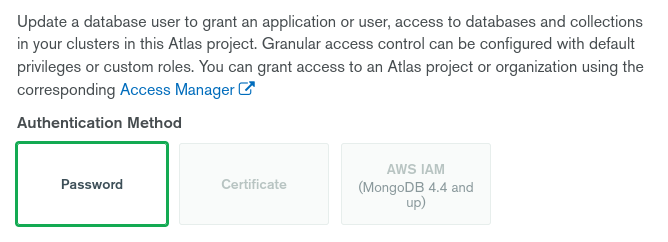
\includegraphics[scale=.5]{./Figures/dbpass.png}
	\caption{Método de autenticación elegido\protect\footnotemark.}
	\label{fig:dbpass}
\end{figure}

\subsection{Comunicación OPC}

Para la comunicación OPC se desarrollo un servicio y se instaló en el mismo nodo virtualizado en donde se ejecuta el sistema de control. Se encarga de actualizar la base de datos según los cambios en el sistema de control. Y viceversa, también es capaz de actualizar las variables de control de acuerdo a la base de datos. Se desarrolló en .NET y se ejecuta como un servicio más de Windows. El servicio incluye el \textit{framework} OPC mencionado en el Capítulo 2, lo que le permite leer y escribir variables OPC. A continuación podemos un extracto de código de la implementación de la interfaz OPC:

\begin{lstlisting}[label=cod:vControl,caption=Implementación de la interfaz OPC]  % Start your code-block

public interface IOpcClient : IDisposable
    {
        bool RefreshGruopAfterCreate { get; set; }
        bool LogSubcriptionsAndWrites { get; set; }
        bool IsServerRunning { get; }
        event ServerShutdownHandler OnServerShutdown;
        void Connect(bool createSubcription);
        void Connect();
        void Disconnect();
        object ReadObject(string idItem);
        string ReadString(string idItem);
        ushort ReadWord(string idItem);      
        void WriteString(string idItem, string value);
        void WriteWord(string idItem, ushort value);
    }
\end{lstlisting}

Podemos ver las funciones principales para leer y escribir, datos booleanos, strings y enteros del servidor OPC del sistema de control.

Una vez que el servicio se encuentra corriendo se encarga de realizar consultas GET a la APIrest de cada una de las recetas en ejecución. De ésta manera es capaz de detectar que los insumos ya fueron vertidos en el tanque y avanzar así a la siguiente etapa. Además, se encarga de setear la variable ``waitinput'', la misma es clave en el funcionamiento de la aplicación dado que indica que la receta se encuentra en ejecución y aguarda órdenes del operador. De ésta manera se valida que el operador sólo pueda iniciar la aplicación con la receta en ejecución por más que intente leer otros códigos de receta inválidos. 

\subsection{Sistema de control}

Este nodo se implementó en una máquina virtual usando VirtualBox, posee un sistema operativo Windows 10 con 4 gb de memoria RAM y 60 Gb de disco. La ventaja radica en la portabilidad del nodo, dado que podría integrarse a un servidor ESXI \citep{esxi} en cualquier entorno industrial. 

En el CBM podemos ver los bloques de las distintas recetas que se crearon en la aplicación de control, como se muestra en la figura \ref{fig:c7}.

\begin{figure}[htpb]
	\centering
	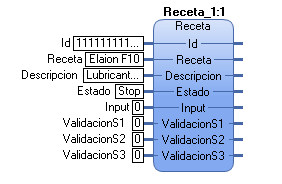
\includegraphics[scale=.6]{./Figures/c7.png}
	\caption{Bloque receta\protect\footnotemark.}
	\label{fig:c7}
\end{figure}

A medida que nuevas recetas sean necesarias, estos bloques funcionan como objetos de una clase que pueden instanciarse para cada tipo de receta. Simultáneamente estas recetas se cargan en la base de datos para establecer la comunicación entre el sistema de control y la interfaz del Hololens 2. Dentro de la receta se puede ver una lógica secuencial del procedimiento, que irá avanzando a medida que el operador complete los pasos en la interfaz holográfica. Podemos ver en la figura \ref{fig:c123} el avance de la secuencia en el tiempo.

\begin{figure}[htpb]
	\centering
	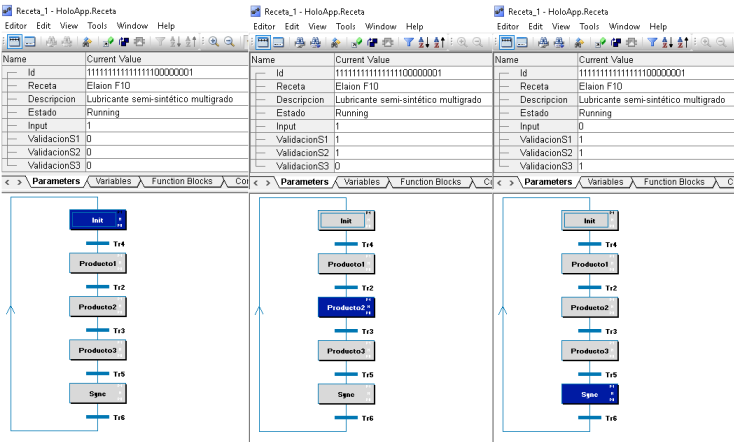
\includegraphics[scale=.5]{./Figures/c123.png}
	\caption{Secuencia\protect\footnotemark.}
	\label{fig:c123}
\end{figure}

La solución propuesta es fácilmente escalable desde la lógica de control y no esta atada a ningún proveedor en particular. Esto se debe a que en cualquier sistema de control somos capaces de crear este clase de objetos y comunicarlos vía el \textit{standard} OPC. Es por eso que el servicio OPC desarrollado, es capaz de operar con distintos sistemas de control sin alterar el funcionamiento de la aplicación desarrollada para el Hololens 2.


% Chapter Template

\chapter{Ensayos y resultados} % Main chapter title

\label{Chapter4} % Change X to a consecutive number; for referencing this chapter elsewhere, use \ref{ChapterX}

%----------------------------------------------------------------------------------------
%	SECTION 1
%----------------------------------------------------------------------------------------

\section{Evaluación de las interfaces}
\label{sec:pruebasHW}

A continuación podemos ver algunas mediciones de tiempos de respuesta de las interfaces principales. Para la medición Hololens - API, se utilizo la opción \textit{debug} del Hololens para identificar el \textit{timestamp} del comando emitido al clickear ``Siguiente'' en la interfaz. Ademas se utilizo la API para loguear el \textit{timestamp} en el que se recibe la consulta web. Para la medición API - server OPC, también se utilizo la API para loguear el \textit{timestamp} en el que se recibe la consulta web. Y se utilizo el servicio OPC para loguear el momento en el que la variable OPC es actualizada. Para un promedio de 10 mediciones consecutivas, los resultados pueden verse en la tabla \ref{tab:interfaces}:

\begin{table}[htpb]
	\centering
	\caption[Tiempos de respuesta]{Tiempos de respuesta promedio}
	\scalebox{0.9}{
	\begin{tabular}{l c c}    
		\toprule
		\textbf{Interfaz} 	 & \textbf{Tiempo}  \\
		\midrule
		Hololens - API				&  >340ms \\		
		API - server OPC	 		&  >320ms \\
		\bottomrule
		\hline
	\end{tabular}}
	\label{tab:interfaces}
\end{table}

Dado que la aplicación se comunica a través de mensajes del tipo JSON y la cantidad de información enviada es reducida, los tiempos de respuesta son realmente bajos y no representan un problema para la implementación. Podemos ver que el tiempo de respuesta de toda la cadena de comunicación, es inferior al segundo. Este trabajo se realizo utilizando servidores \textit{cloud} pero bien podrían ser locales. Llegado el caso, si los tiempos representan una perdida de fluidez en la aplicación, la migración no requeriría mayores esfuerzos. 
 
% Chapter Template

\chapter{Conclusiones} % Main chapter title

\label{Chapter5} % Change X to a consecutive number; for referencing this chapter elsewhere, use \ref{ChapterX}


%----------------------------------------------------------------------------------------

%----------------------------------------------------------------------------------------
%	SECTION 1
%----------------------------------------------------------------------------------------

\section{Resultados obtenidos}

Fue muy importante la planificación inicial para enmarcar y organizar el trabajo. Las estimaciones fueron correctas, aunque se subestimo la etapa de integración de todos los componentes. El trabajo se extendió hasta el mes de Junio solapándose con la redacción de la tesis. 

El trabajo respeto los requerimientos propuestos, pero no se logro una robustez en cuanto a la seguridad informática. En principio, estaba pensada la utilización de un \textit{token} de seguridad para la API pero fue desestimado conforme avanzaba el proyecto. Principalmente porque mientras la conexión no sea encriptada la utilización del \textit{token} carece de sentido. Esto es algo que se plantea como una mejora a futuro.

El trabajo logro integrar realidad aumentada, plataformas \textit{cloud} y sistemas de control tradicionales con éxito. La aplicación resulto útil en las pruebas realizadas, y durante las presentaciones con clientes industriales el \textit{feedback} fue positivo. El trabajo demostró que las integraciones de sistemas de control con las tecnologías 4.0 son posibles, pero es necesario encontrar casos de uso prácticos que justifiquen el esfuerzo del desarrollo. La mano de obra no solo puede automatizarse, sino que también puede mejorarse con ayuda de las nuevas tecnologías.

%----------------------------------------------------------------------------------------
%	SECTION 2
%----------------------------------------------------------------------------------------
\section{Próximos pasos}

El siguiente paso es utilizar un \textit{token} para autenticar la comunicación y certificados TLS  para encriptar el canal de comunicación entre el Hololens y el servidor web. De esta manera se mejoraría la seguridad considerablemente. Utilizando ademas lo desarrollado, se tiene el punto de partida para realizar una segunda aplicación orientada al mantenimiento de activos en la planta.
 

%----------------------------------------------------------------------------------------
%	CONTENIDO DE LA MEMORIA  - APÉNDICES
%----------------------------------------------------------------------------------------

\appendix % indicativo para indicarle a LaTeX los siguientes "capítulos" son apéndices

% Incluir los apéndices de la memoria como archivos separadas desde la carpeta Appendices
% Descomentar las líneas a medida que se escriben los apéndices

%\include{Appendices/AppendixA}
%\include{Appendices/AppendixB}
%\include{Appendices/AppendixC}

%----------------------------------------------------------------------------------------
%	BIBLIOGRAPHY
%----------------------------------------------------------------------------------------

\Urlmuskip=0mu plus 1mu\relax
\raggedright
\printbibliography[heading=bibintoc]

%----------------------------------------------------------------------------------------

\end{document}  
